\documentclass[12pt]{article}

\usepackage[a4paper,left=25mm,right=25mm,top=35mm,bottom=25mm]{geometry}
\usepackage{ngerman}
\usepackage{parskip}
\usepackage{times}
\usepackage{graphicx}
\usepackage{listings}
\usepackage{fancyhdr}
\usepackage{float}
\usepackage{amsmath}

\setlength{\headheight}{15.2pt}
\pagestyle{fancy}

\lhead{Bildverarbeitung und Mustererkennung\\Praktikum Blatt 8}
\rhead{Patrick Hüntelmann\\10.06.2022}

\lstset{
  basicstyle=\ttfamily,
  breakatwhitespace=false,         % sets if automatic breaks should only happen at whitespace
  breaklines=true,                 % sets automatic line breaking
  captionpos=b,                    % sets the caption-position to bottom
  deletekeywords={...},            % if you want to delete keywords from the given language
  escapeinside={\%*}{*)},          % if you want to add LaTeX within your code
  extendedchars=true,              % lets you use non-ASCII characters; for 8-bits encodings only, does not work with UTF-8
  frame=single,	                   % adds a frame around the code
  keepspaces=true,                 % keeps spaces in text, useful for keeping indentation of code (possibly needs columns=flexible)
  language=python,                 % the language of the code
  showstringspaces=false,          % underline spaces within strings only
  showtabs=false,                  % show tabs within strings adding particular underscores
  tabsize=2,	                   % sets default tabsize to 2 spaces
}

\begin{document}

\pagenumbering{arabic}

\section*{Aufgabe 8}
\subsection*{a) Hough-Transformation für Kreise}
Die Hough-Transformation für Kreise ist in der Funktion \textbf{hough\_circles} (main.py Zeile 22) implementiert.
Diese Funktion bekommt als Parameter das Kantenbild, sowie den minimalen und maximalen Radius übergeben und gibt anschließend eine Liste zurück in der die Mittelpunkte der gefundenen Kreise sowie der Radius des Kreises angegeben ist.

\subsection*{b) Münzen lokalisieren}
Nach der Suche der Kreise werden die Ergebnisse anhand des Radius des Kreises in verschiedene Kategorien (1 Cent, 2 Cent oder 5 Cent Münze) unterteilt. (main.py Zeile 72)
Anschließend wird auf dem Ausgangsbild eine Umrandung für jeden Kreis gezeichnet und der Mittelpunkt markiert.

\subsection*{c) Münzen zählen}
Anhand der Kategorie des Kreises wird ein Zähler um den entsprechenden Wert (1 für 1 Cent, 2 für 2 Cent und 5 für 5 Cent) inkrementiert. Zum Schluß wird das Ergebnis ausgegeben (main.py Zeile 88).

\subsubsection*{Ergebnisbilder}
\begin{figure}[H]
  \centering
  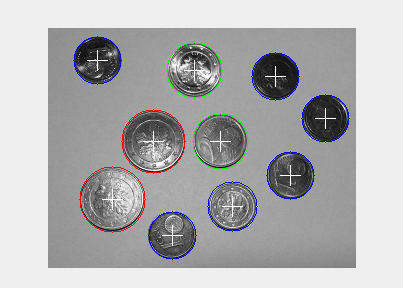
\includegraphics[width=0.7\textwidth, keepaspectratio]{hough.png}\\
  Ergebnisbild mit Umrandung der Münzen und markiertem Mittelpunkt 
\end{figure}
\begin{figure}[H]
  \centering
  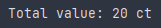
\includegraphics[width=0.4\textwidth, keepaspectratio]{total.png}\\
  Summe der Münzen
\end{figure}

\end{document}
